\section[Itération~3:~(~4/3/2017~-~4/28/2017~)]{Itération~3:~\textup{\textto{(~4/3/2017~-~4/28/2017~)}}}

\subsection{Introduction}

Dans la dernière itération, nous avons collecté un grand ensemble de donnés des
différents types.  Malgré tout, ces donnés n'ont pas de valeur tel que on les
explore pas. C'est le rôle du Business Intelligence que nous allons étudier
dans cette itération.

\subsection{L'objectif du sprint}

En accord avec le product owner,le but de cette itération est:

\begin{description}
    \item [Smartphone] L’ajout de nouvelles fonctionnalités comme:
        \begin{itemize}
            \item La détection des réseaux avec leur intensité.
            \item l'exploitation des donnes collecté selon le besoin.
        \end{itemize}
    \item [Rapport] Typage des rapports.
    \item [Dashboard] \textbf{}

        \begin{itemize}
            \item Élaboration des mécanisme d'authentification.
            \item Des nouveaux marqueurs qui spécifient chaque type de rapport
                ajouté.
        \end{itemize}
\end{description}

%Le Product Owner nous a demandé d’améliorer le chargement de l'image
%dans le serveur de telle sorte que la qualité d'image reste la même..
%Donc, dans cette itération, nous allons tenir compte des attentes du Product Owner. Nous allons
%modifier le critère de chargement, En plus nous allons implémenter une méthode
%permettant de maintenir la qualité.

\subsection{Planification de l'itération 3}

\subsubsection{Backlog de l'itération}

On définit dans le tableau~\ref{tab:sprint3-backlog} la liste de nos taches
dans cette itération.

\begin{center}
    \footnotesize
    \begin{longtable}{| p{1cm} | p{5cm} | p{7cm} | p{1cm} |}
        \caption{Taches à faire de la troisième itération}
        \label{tab:sprint3-backlog} \\

 \hline
 \multicolumn{1}{|c}{\textbf{Réf}} &
 \multicolumn{1}{|c}{\textbf{Spécification}} &
 \multicolumn{1}{|c}{\textbf{Description}} &
 \multicolumn{1}{|c|}{\textbf{Priorité}} \\ \hline
 \endhead

 \hline \multicolumn{4}{|r|}{{Continué en page suivante$\dotsc$}} \\ \hline
 \endfoot

 \hline \hline
 \endlastfoot

\hline
3.1 & Integration Dashboard et Rapport dans l'application android & Implémenté la méthode qui affiche les pages ``Dashboard et Rapport'' chacun a un bouton spécifié   & 1 \\ \hline
3.2 & Authentification Restful  & Ajouter l'authentification dans le serveur pour assurer la sécurité   & 1 \\ \hline
3.3 & landing page & créer une nouvel page Web  & 3\\ \hline
3.4 & Compte utilisateur & Base de données accecible depuis l'application et le web& 2 \\ \hline
3.5 & Post réseau & Methode POST Restful & 1 \\ \hline
3.6 & GET réseau & Methode GET Restful & 1 \\ \hline
3.7 & Post vitesse & Methode POST vitesse & 1 \\ \hline
3.8 & Get vitesse & Methode GET & 1 \\ \hline
3.9 & Appplication Android Responsive & Responsive design coter android & 3 \\ \hline
3.10 & IHM & l'ajout des boutons radio pour distinguer (pieton / voiture)(android) & 3 \\ \hline
3.11 & Recherche Business intelligence & BI & 2 \\ \hline
3.12 & Implantation des BD au BI & données accessible en BI & 2\\ \hline
3.13 & création Logo &Ajouter Logo dans l'application & 3 \\ \hline
3.14 & étude scénario commercial embouteillage & scénario de marketing& 2\\ \hline
3.15 & Rectification chargement image & \ldots & 1 \\ \hline
3.16 & étude scénario commercial secousses & scénario de marketing& 2\\ \hline
\end{longtable}
\end{center}

\subsubsection{Estimation de la deuxième itération}

Le tableau~\ref{tab:sprint3-capacity} représente l'estimation du nombre
d'heures pendant lesquelles nous nous engageons à travailler dans une période
de 3 semaines.

\begin{table}[htbp]
    \centering
    \begin{tabular}{| c | c | c | c |}
\hline
\textbf{Membre} & \textbf{Nombre d'heures par jour} & \textbf{Nombre de jours présent} & \textbf{Total en heures} \\ \hline
\hline

Moez & 8 & 48 & 144\\ \hline
Rihab & 8 & 48 & 144 \\ \hline
\multicolumn{2}{c|}{} & \textbf{Total} & 288 \\ \cline{3-4}
    \end{tabular}
    \caption{Nombre d'heures de travail estimé de l'itération 3}
    \label{tab:sprint3-capacity}
\end{table}

Le tableau~\ref{tab:sprint3-estimation} représente les estimations de nos taches
en heures pour cette itération.

\begin{center}
    \begin{longtable}{| l | l | l |}
        \caption{Nombre d'heures estimé pour la réalisation des taches}
        \label{tab:sprint3-estimation} \\

 \hline
 \multicolumn{1}{|c}{\textbf{Spécification}} &
 \multicolumn{1}{|c}{\textbf{Membre}} &
 \multicolumn{1}{|c|}{\textbf{Heures}} \\ \hline
 \endhead

 \hline \multicolumn{3}{|r|}{{Continué en page suivante$\dotsc$}} \\ \hline
 \endfoot

 \hline \hline
 \endlastfoot

\hline
Integration Dashboard et Rapport dans l'application android & Rihab & 5 x 2 \\ \hline
Authentification Restful& Rihab \& Moez & 13 x 2 \\ \hline
landing page& Rihab & 13 \\ \hline
Compte utilisateur& Moez & 8 \\ \hline
Post réseau& Moez & 5  \\ \hline
GET réseau& Moez & 5  \\ \hline
Post vitesse& Rihab & 5  \\ \hline
Get vitesse& Rihab & 5  \\ \hline
Appplication Android Responsive & Rihab & 13 \\ \hline
IHM & Rihab & 5 x 2 \\ \hline
Recherche Business intelligence& Moez & 13 x 2 \\ \hline
Implantation des BD au BI& Moez & 13 x 2 \\ \hline
création Logo& Rihab & 13 \\ \hline
Étude scénario commercial embouteillage& Rihab & 13 x 2 \\ \hline
Rectification chargement image & Rihab & 13 x 2 \\ \hline
Étude scénario commercial secousses & Rihab & 13 x 2 \\ \hline
\end{longtable}
\end{center}

\subsection{Présentation des outils utilisés}

\subsubsection{OAuth2}

\TODO{what is it, alternatives, why}

% Les API REST sont basées sur le protocole HTTP, qui signifie Hypertext Transfer Protocol.
% C’est ce qui est au cœur du web! C’est un protocole qui définit la communication
% entre les différentes parties du web. L’échange est basé sur des requêtes client et serveur.
% Un client lance une requête HTTP, et le serveur renvoie une réponse.
% Ce sont des méthodes qui définissent les requêtes que le client peut effectuer,
% dont GET\footnote{Récupérer une ressource (ne modifie pas la ressource).}, PUT\footnote{Modifier une ressource.},
% POST\footnote{Créer une ressource.}, DELETE\footnote{Supprimer une ressource.} encore plus.

\subsubsection{Business Intelligence}

La \acrfull{BI}\footnote{Informatique décisionnelle} propose d'utiliser les
données transitant par le Système d'information en informations susceptibles
d'être exploitées à des fins décisionnelles.

% Sur le plan pratique et technique, la Business Intelligence se compose d'une
% famille d'outils informatiques et de progiciels assurant le fonctionnement de
% la chaîne de traitement de l'information.

Les 4 fonctions de la chaîne décisionnelle:

% comment s'explique la
% figure~\ref{fig:sprint3-businessintelligence} sont:

\begin{description}
    \item [\acrfull{ETL}] Collecter, nettoyer et consolider les données
        Extraire les données des systèmes de production et les adapter à un
        usage décisionnel.
    \item [\acrfull{DW}] Stocker Centraliser les données structurées et
        traitées afin qu'elles soient disponibles pour un usage décisionnel.
%    \item [??] Distribuer Ou plutôt faciliter l'accessibilité des informations
%        selon les fonctions et les types d'utilisation.
    \item [\acrfull{OLAP}] Exploiter ou comment assister du mieux possible
        l'utilisateur afin qu'il puisse extraire la substance de l'information
        des données stockées à cet usage.
    \item [Rapports] Des rapports sont générés sur ces différents données
        traitées. Les rapports peuvent être des rapports traditionnels composés
        des tableaux ou des rapport visuels composés des diagrammes et cartes
        dynamiques ou statiques d’une manière synthétique ou détaillée. Ces
        rapports sont ensuite utilisé par les décideurs et les dirigeants pour
        prendre des décisions.
\end{description}

Dans notre projet, le Product Owner et les participants au projet nous avons
recommandé d'explorer la solution du Microsoft du BI grâce aux compétences du
nos encadreurs dans cette technologie. Les outils du Microsoft BI qu'on avait
utilisés au cours de cette itération sont:

\begin{description}
    \item [\acrfull{SSIS}] La solution du Microsoft pour l'\acrshort{ETL}. Elle
        permet d'extraire et d'importer aisément les donnée à un ou des bases
        de données du serveur SQL Server.
    \item [MS Power BI] Permettre de générer des tableaux du bord des rapports
        visuels et dynamiques accessible en ligne facilement et sans besoin du
        codage. C'est une solution alternative de \acrfull{SSRS}.
\end{description}
%\clearpage

%\begin{figure}[htbp]
%  \centering
%  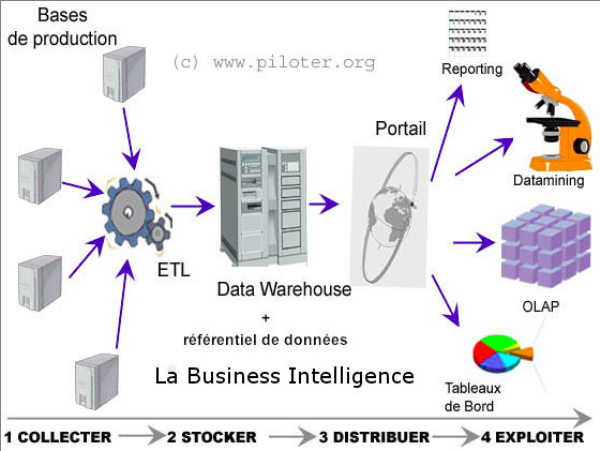
\includegraphics[width=0.8\textwidth]{sprint3-businessintelligence}
%  \caption{Les 4 phases du processus de Business Intelligence}
%  \label{fig:sprint3-businessintelligence}
%\end{figure}

\subsection{Mises des normes}

Les critères à respecter pendant cette itération incluent les même critères de
l'itération 1 et de plus:

\begin{description}
    \item [Sécurité] L'implémentation de l'authentification doit être sécurisée
        de tel façon, on ne peut pas accéder au contenu protégé sans
        authentification.
    \item [Permissions] Un utilisateur n'a la permission que de changer ses
        donnés personnelles et n'a pas l'autorisation d'accès au donnés privé
        de les autres (trajet, détails de contact, \ldots).
    \item [Visualisation Instantané des Statistiques] Les diagrammes de
        statistiques doivent mets à jour instantanément et continuellement.
\end{description}

\subsection{Conception}

la figure~\ref{fig:sprint3-webservices-oauth-usecase} décrit le diagramme
de cas d'utilisation de service d'authentification.

\begin{figure}[htbp]
    \centering
    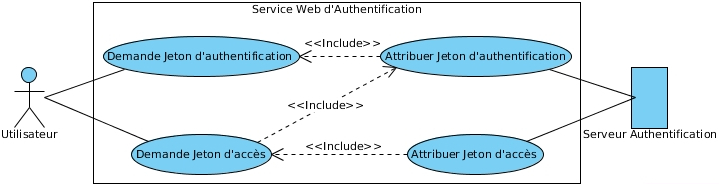
\includegraphics[width=1\textwidth]{sprint3-webservices-oauth-usecase}
    \caption{Diagramme de case d'utilisation du service d'Authentification en itération 3}
      \label{fig:sprint3-webservices-oauth-usecase}
\end{figure}

la figure~\ref{fig:sprint3-webservices-oauth-sequence} présente le diagramme de
séquence du services d'authentification.

\begin{figure}[htbp]
    \centering
    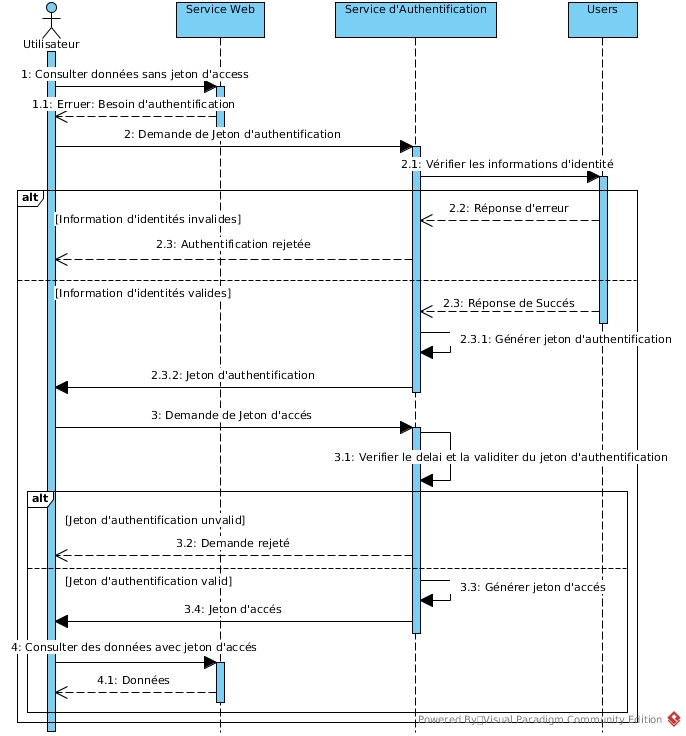
\includegraphics[width=1\textwidth]{sprint3-webservices-oauth-sequence}
    \caption{Diagramme de sequence du services d'authentification en itération 3}
    \label{fig:sprint3-webservices-oauth-sequence}
\end{figure}

la figure~\ref{fig:sprint3-webservices-database} représente notre base de
donnes de la troisième itération.

\begin{figure}[htbp]
    \centering
    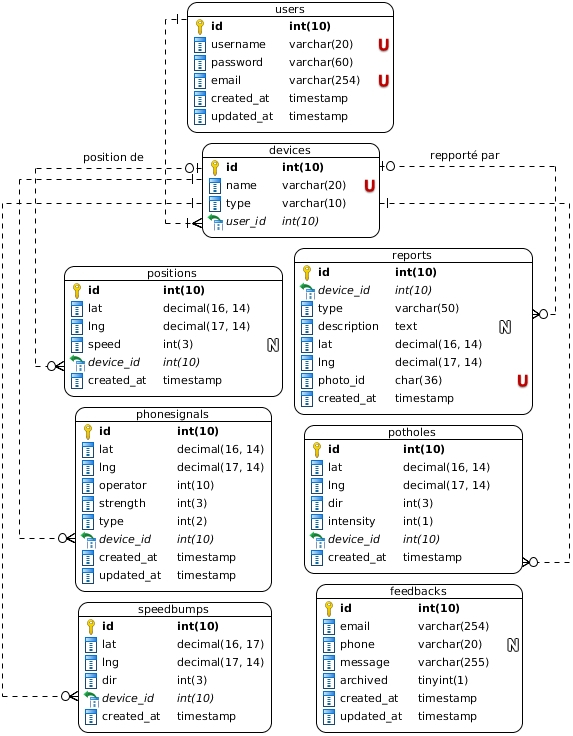
\includegraphics[width=1\textwidth]{sprint3-webservices-database}
    \caption{Diagramme d'entité-relation du services web en itération 3}
    \label{fig:sprint3-webservices-database}
\end{figure}

la figure~\ref{fig:sprint3-dashboard-classs} décrit le diagramme des classes du
page \textquote{Dashboard} dans la troisième itération.

\begin{figure}[htbp]
    \centering
    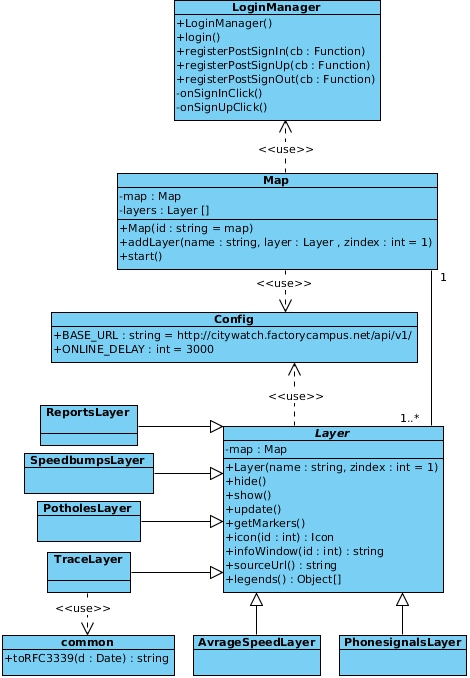
\includegraphics[width=1\textwidth]{sprint3-dashboard-class}
    \caption{Diagramme des classes du Dashboard en itération 3}
    \label{fig:sprint3-dashboard-classs}
\end{figure}

\subsection{Évaluation suivant les normes mise}

\TODO{}

\subsection{Revue de cette itération}

% On rappelons que nous travaillons dans un équipe Scrum qui nécessite
% l'intégration de notre travail dans le projet pour attendre le but.

\subsubsection{Produit de l'itération}

\paragraph{Légende du Dashboard}
Dans cette page nous travaillons alors sur deux parties:

\begin{itemize}
    \item la première: active/désactive les boutons de filtrage de chaque
        marqueur.
    \item la deuxième: gérés la communication interne entre serveur et la page.
\end{itemize}

Aussi, nous participons 80\% à l'ajout de légende a notre carte et affiche le
filtrage des marqueurs.

\begin{figure}[htbp]
\centering
    \begin{subfigure}{.8\textwidth}
    \centering
  \centering
  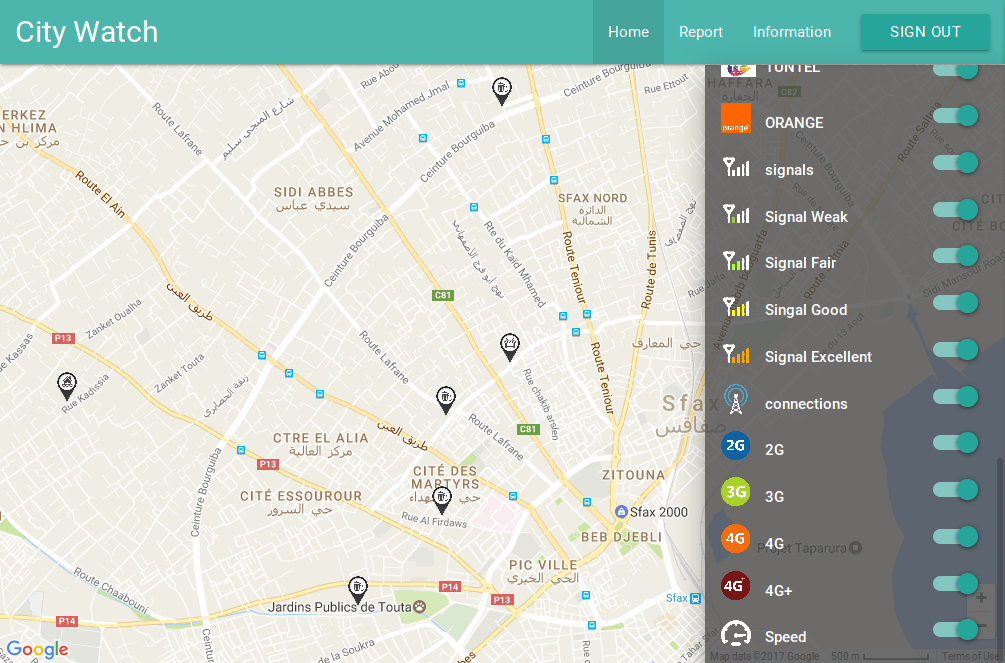
\includegraphics[width=1.0\linewidth]{sprint3-dashboard-screenshot1}
  \caption{Marqueurs activé}
  \label{fig:sprint3-dashboard-screenshot1}
\end{subfigure}
\begin{subfigure}{.8\textwidth}
    \centering
  \centering
  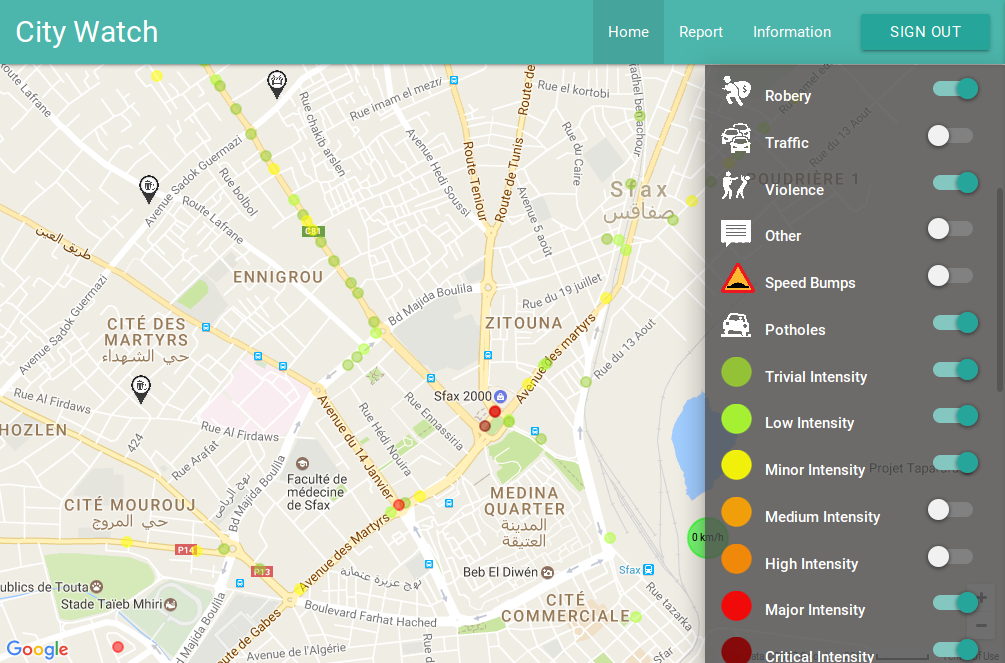
\includegraphics[width=1.0\linewidth]{sprint3-dashboard-screenshot2}
  \caption{Quelques marqueurs désactivé}
  \label{sprint3-dashboard-screenshot2}
\end{subfigure}
\caption{Dashboard CityWatch au troisième itération}
\end{figure}
\clearpage

\paragraph{Android}

\paragraph*{}
Les données captées par l'application mobile (Position , Secousses , Ralentisseur , Réseaux , force du 
signal et vitesse ) sont Récupérées par le serveur pour assurer la sauvegarde et la transmission vers une 
base données.\\

\begin{figure}[htbp]
\centering
    \begin{subfigure}{.45\textwidth}
    \centering
  \centering
  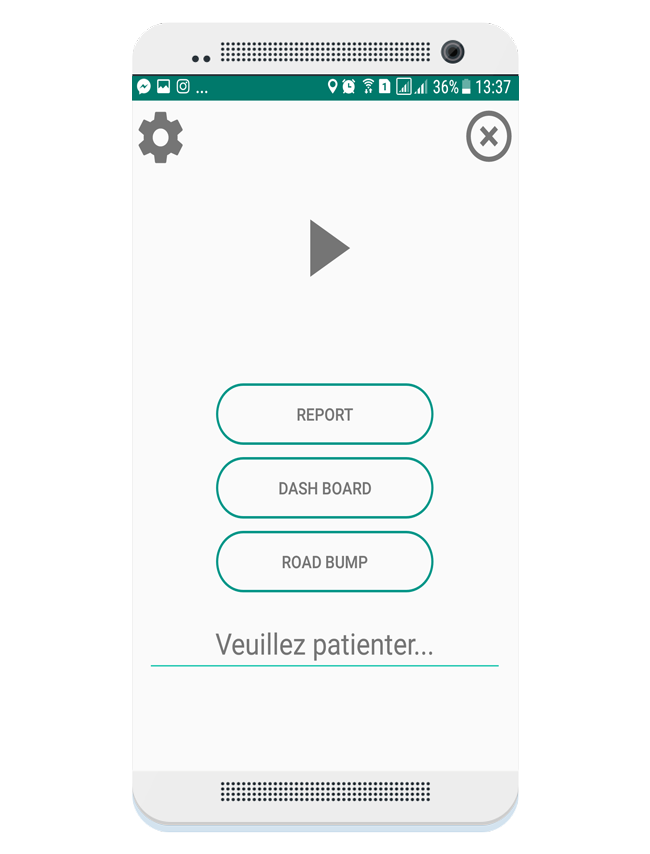
\includegraphics[width=1.0\linewidth]{sprint3-android-screenshot1}
  \caption{État désactivé}
  \label{fig:sprint3-android-screenshot1}
\end{subfigure}
\begin{subfigure}{.45\textwidth}
    \centering
  \centering
  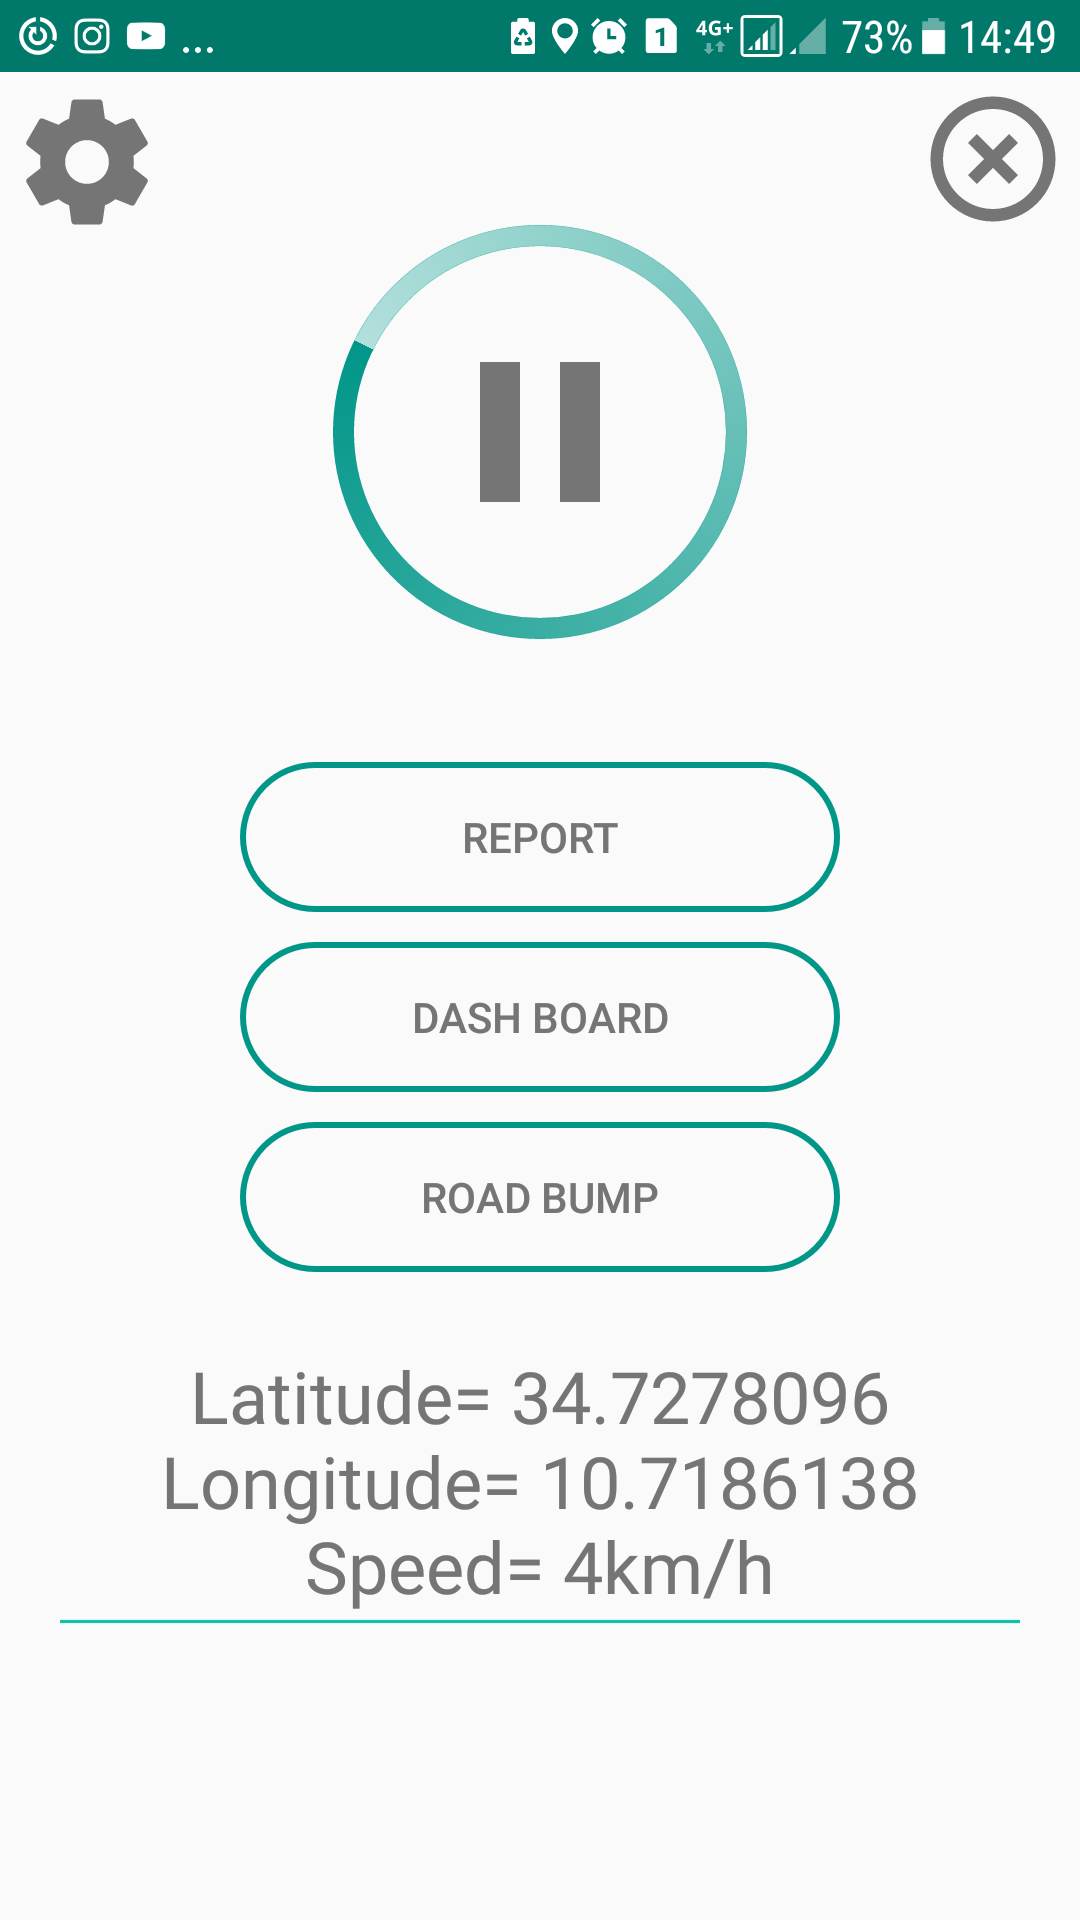
\includegraphics[width=1.0\linewidth]{sprint3-android-screenshot2}
  \caption{État activé}
  \label{fig:sprint3-android-screenshot2}
\end{subfigure}
\caption{Interface de l'application au troisième itération}
\end{figure}
\clearpage

\subsubsection{Avis du Product Owner}

Après la présentation du produit final, le \textquote{Product Owner} était très satisfait
a notre travail.

\subsubsection{Burndown chart}

La figure~\ref{fig:sprint3-burndown} présente une vue d'ensemble sur le progrès
de notre travail au cours de l'itération par rapport au progrès idéal.

\usetikzlibrary{plotmarks}

\begin{figure}
\centering
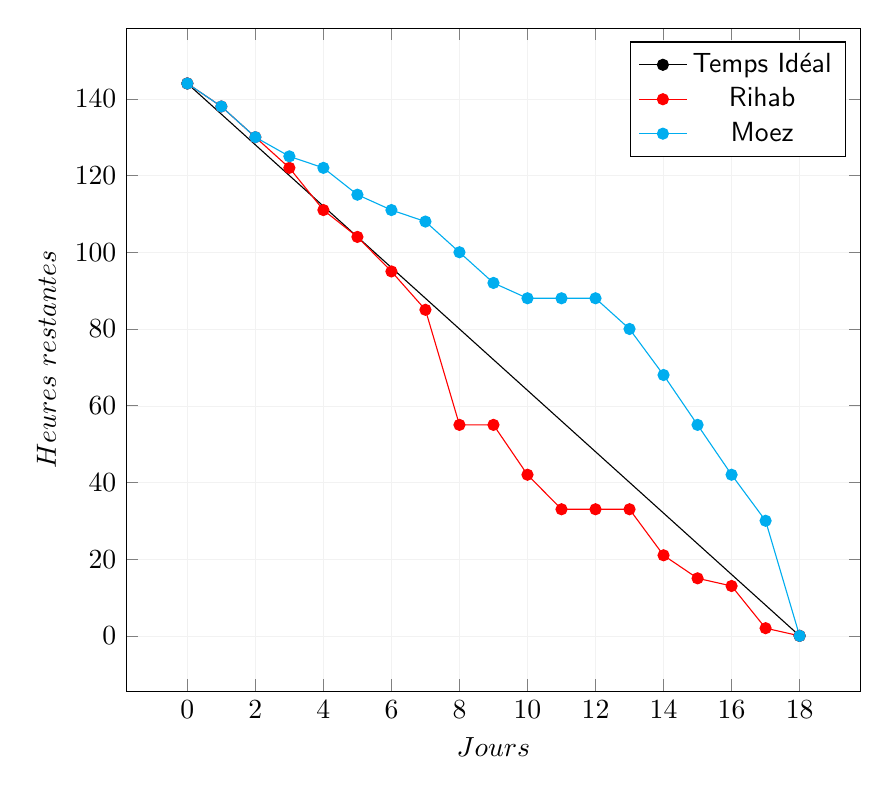
\begin{tikzpicture}[y=.2cm, x=.7cm,font=\sffamily]
\begin{axis}[
xlabel=$Jours$,
ylabel=$Heures\ restantes$,
grid=both,
grid style={line width=.1pt, draw=gray!10},
width=0.9\textwidth,
height=10cm,
%major grid style={line width=.2pt,draw=gray!50},
]
\addplot[color=black,mark=*] coordinates {
        (0,144)
        (18,0)
    };
    \addlegendentry{Temps Idéal}

    \addplot[mark=*,red] plot coordinates {
        (0, 144)
        (1, 138)
        (2, 130)
        (3, 122)
        (4, 111)
        (5, 104)
        (6, 95)
        (7, 85)
        (8, 55)
        (9, 55)
        (10, 42)
        (11, 33)
        (12, 33)
        (13, 33)
        (14, 21)
        (15, 15)
        (16, 13)
        (17, 2)
        (18, 0)
       
    };
    \addlegendentry{Rihab}
      \addplot[mark=*,cyan] plot coordinates {
       (0, 144)
        (1, 138)
        (2, 130)
        (3, 125)
        (4, 122)
        (5, 115)
        (6, 111)
        (7, 108)
        (8, 100)
        (9, 92)
        (10, 88)
        (11, 88)
        (12, 88)
        (13, 80)
        (14, 68)
        (15, 55)
        (16, 42)
        (17, 30)
        (18, 0)
       
    };
    \addlegendentry{Moez}
\end{axis}
\end{tikzpicture}
\caption{Graphique d'avancement - Itération 3}
\end{figure}


\subsection{Conclusion}

A fin de cette itération, nous avons découvert des nouveaux aspects intéressants dans notre projet
qui nécessitent l'intervention des technologies (big-data, data mining, \ldots).

Le tableau~\ref{tab:sprint3-evaluation} présente le pourcentage de
réalisation de nos taches de cette itération.

\begin{center}
    \begin{longtable}{| l | l |}
        \caption{Liste des tâches réalisées de la troisième itération}
        \label{tab:sprint3-evaluation} \\

        \hline
        \textbf{Les tâches} & \textbf{Taux de réalisation} \\ \hline
        \endhead

        \hline \multicolumn{2}{|r|}{{Continué en page suivante$\dotsc$}} \\ \hline
        \endfoot

        \hline \hline
        \endlastfoot

        \hline
Integration Dashboard et Rapport dans l'application android & Effectué 100\% \\ \hline
Authentification Restful&  Effectué 100\% \\ \hline
landing page& Effectué 100\% \\ \hline
Compte utilisateur& Effectué 100\% \\ \hline
Post réseau& Effectué 100\% \\ \hline
GET réseau&  Effectué 100\% \\ \hline
Post vitesse&  Effectué 100\% \\ \hline
Get vitesse& Effectué 100\% \\ \hline
Appplication Android Responsive & Effectué 100\% \\ \hline
IHM & Effectué 100\% \\ \hline
Recherche Business intelligence& Effectué 100\% \\ \hline
Implantation des BD au BI & Effectué 30\% \\ \hline
création Logo&  Effectué 80\% \\ \hline
Étude scénario commercial embouteillage& Effectué 100\% \\ \hline
Rectification chargement image & Effectué 100\% \\ \hline
Étude scénario commercial secousses &  Effectué 100\% \\ \hline
\end{longtable}
\end{center}
